\documentclass[11pt]{article}
\usepackage[margin=1in]{geometry}
\usepackage{amsmath,amssymb,booktabs,graphicx,array}
\usepackage[colorlinks=true,urlcolor=blue,citecolor=blue]{hyperref}
\setlength{\emergencystretch}{3em}
\newcommand{\F}{\mathbb{F}}
\newcommand{\Acc}{\operatorname{Acc}}
\title{When Does Correct Relational Geometry Support Unseen Composition?}
\author{}
\date{}
\begin{document}
\maketitle
\begin{abstract}
We study whether the correctness of supplied mathematical state correspondences supports unseen composition when correct output supervision is fixed. In a final finite-matrix confirmation with five new source initializations and relation-prepared frozen encoders, a parameter-matched activation-by-correctness intervention yields a 12.89 percentage-point interaction. Transferring predicted readout-null components from correctly trained GELU operators improves a linear recipient by 8.75 points while preserving all first-step logits. Adequate affine fitting under the identical single-step loss recovers most of the functional correspondence benefit; the remaining interaction is 0.31 points with a descriptive interval crossing zero. Ill-conditioning and precision sensitivity qualify that optimization result. Permutation experiments provide a second correspondence-sensitive setting, while initial matrix, polynomial, and null-only-loss studies establish boundaries. The evidence supports a conditional functional pathway and an optimization-sensitive interpretation, without establishing spontaneous algebra discovery, robust hidden-relation inference, or a universal output-independent mechanism.
\end{abstract}

\section{Introduction}
Exact input transformations provide a controlled way to study what a neural representation preserves. A task answer may transform predictably when an input is inverted, complemented, translated, or differentiated. Yet matching transformed answers, aligning hidden vectors, and predicting an unseen composition are different achievements. A representation can support an accurate first-step answer while omitting information required by the next operation.

We ask whether \emph{the correctness of a supplied state correspondence} improves held-out composition when output supervision is held fixed. The distinction matters because geometric supervision ordinarily changes both the state target and the answer information available during training. We use exact finite mathematical worlds to construct incorrect correspondences that preserve visible gold answers, endpoint marginals, input exposure, and correct teacher-output supervision. The intervention changes which intermediate hidden state is treated as the geometric target.

Our primary evidence comes from a final confirmation with five new source initializations in a finite matrix world. Encoders first receive ordinary task training and correct single-generator preparation. We then freeze each encoder, its second operator, and its readout, and cross first-operator activation with correct versus matched-incorrect correspondence. This is a conditional intervention on relation-prepared representations. It does not test whether ordinary training discovers algebra spontaneously.

Three findings form the paper's argument. First, under a fixed budget, correctly paired GELU operators support more accurate unseen composition than their matched-incorrect counterparts. Second, predicted components invisible to the fixed first-step linear readout can transmit this benefit: swapping those components improves a linear recipient while preserving every first-step logit. Third, adequately fitting the same affine function family under the same single-step objective recovers most of the functional correctness benefit. Consequently, the original budget-controlled nonlinear advantage does not establish an additional expressivity advantage.

Permutation studies provide a second instance of correspondence-sensitive composition and motivate the intermediate-state diagnostics. Initial joint affine matrix experiments, an irreversible polynomial experiment, and a null-only-loss intervention establish important boundaries. Their architectures, supervision directions, source counts, and fitting budgets differ; they are supporting studies, rather than a pooled cross-domain confirmation of one universal mechanism.

The contribution is a controlled empirical account of \emph{when geometric correspondence is functionally useful and how that conclusion can be checked}. It combines answer-matched correspondence interventions, predicted-component transfer, independent-source confirmation, and same-family convergence diagnostics. Readers interested in compositional representation learning can use this combination to distinguish answer preservation, downstream state sufficiency, and finite-budget optimization. We make no claim that each diagnostic alone is new, or that the resulting mechanism holds across all mathematical systems.

\section{Related work}
\paragraph{Task relations and representation geometry.}
Turner and Barak \cite{turner2023} study shared attractors and reuse of dynamics in multitask RNNs, including a family of function tasks whose geometry depends on task requirements. Park \cite{park2026} finds representational convergence under multitask city-geometric training, together with task-dependent failures of new-entity integration. These findings motivate separating geometric similarity from functional generalization. Our intervention fixes the source model and correct output targets within each comparison, then changes the correctness of intermediate-state pairing.

\paragraph{Transforming tasks and testing composition.}
Lampinen and McClelland \cite{lampinen2020} learn metamappings that transform task representations to support novel tasks, including polynomial task transformations. Lake and Baroni \cite{lake2018} use SCAN to distinguish successful local generalization from systematic reuse of familiar primitives. Both establish that relationship learning and composition are substantive existing research directions. We study transformations of \emph{input-state representations} with a fixed task readout, and evaluate operator compositions whose endpoint labels and states are absent from fitting.

\paragraph{Equivariance and learned algebraic structure.}
Cohen and Welling \cite{cohen2016} incorporate known symmetries through group-equivariant convolution. Keurti et al.\ \cite{keurti2023} learn group-structured latent representations with a Homomorphism AutoEncoder and evaluate action sequences. Their theoretical justification uses two-step latent prediction together with reconstruction. Our compound endpoint is held out from the single-step fitting objective, and our encoders have no hard-coded group operations. Chughtai et al.\ \cite{chughtai2023} identify representation-theoretic circuits in networks trained for finite-group composition and validate them through ablations. Hwang and Park \cite{hwang2026} relate intrinsic task symmetry, geometric organization, and algorithmic generalization. We provide no circuit recovery or symmetry-acquisition theorem; the question is the functional increment of a controlled correspondence intervention.

\paragraph{Structural diagnostics and latent operators.}
An and Du \cite{an2026}, in a NeurReps workshop paper, use representational homomorphism error to predict synthetic-language compositional generalization. Here an operator prediction error is accompanied by correctness interventions and frozen downstream tests, so a low error alone is not the functional conclusion. Azencot et al.\ \cite{azencot2020} connect forward/backward consistency and Koopman latent dynamics to sequence forecasting. Our affine convergence diagnostic retains the same empirical single-step loss as the original linear arm; it does not introduce a consistency objective or claim to recover a Koopman representation.

\paragraph{Similarity measures and the scope of the comparison.}
Kornblith et al.\ \cite{kornblith2019} develop CKA for comparing representations. Davari et al.\ \cite{davari2022} show that its value can change substantially while functional behavior is largely retained. We therefore treat CKA as auxiliary and prioritize composition accuracy, pairwise success, and controlled state interventions. The closest comparisons are summarized in Table~\ref{tab:related}; they define the question added by this study, not empirical claims of superiority over those methods. The related methods are not reimplemented as competing baselines, and we do not claim priority for learning latent algebra or predicting compositions.

\begin{table}[ht]
\centering\small
\begin{tabular}{p{.23\linewidth}p{.31\linewidth}p{.37\linewidth}}
\toprule
Prior setting & Established focus & Question addressed here\\\midrule
Metamappings \cite{lampinen2020} & Learned transformations between task representations & What changes when state correspondence changes but correct output supervision stays fixed?\\
Homomorphism AutoEncoder \cite{keurti2023} & Equivariant latent actions and sequence prediction & How much composition benefit arises without fitting the held-out compound endpoint?\\
Finite-group circuits \cite{chughtai2023} & Representation-theoretic computation and ablation & Can a predicted state component transmit correspondence-sensitive functional gains?\\
Homomorphism error \cite{an2026} & Structural error as a generalization predictor & Does a correspondence intervention change actual downstream prediction?\\
Task/world geometry \cite{turner2023,park2026,hwang2026} & Geometry associated with task structure or symmetry & Which observed gains survive fixed-output and optimization controls?\\
\bottomrule
\end{tabular}
\caption{Positioning of the controlled empirical question. These are conceptual comparisons, not a performance ranking.}\label{tab:related}
\end{table}

\section{Controlled correspondence and the final confirmation}
\subsection{Prediction problem}
Let $h(x)\in\mathbb{R}^{d}$ be a row-vector representation and let the task logits be
$z(h)=hW^\top+b_W$. Two specified input operations are $T_A$ and $T_B$.
The word $AB$ means \emph{first $A$, then $B$}. Prediction starts from $h(x)$ and produces
\[
 \widehat z_{AB}(x)=z\!\left(R_B(R_A(h(x)))\right).
\]
The program supplies the operation order. It does not compute the mathematical endpoint for the predictor, and the predictor does not forward $T_BT_Ax$ through the encoder. A separate endpoint forward is used only to construct evaluation truth and diagnostics.

\subsection{Exact matrix world and held-out data}
Inputs are the $26{,}208$ invertible $2\times2$ matrices over $\F_{13}$.
The task is $\operatorname{tr}(X)\bmod13$, and left actions use
\[
A=\begin{pmatrix}0&1\\1&0\end{pmatrix},\qquad
B=\begin{pmatrix}0&-1\\1&-1\end{pmatrix}.
\]
They generate a six-element noncommutative group with $A^2=B^3=e$ and $ABA=B^2$.
The action on invertible matrices is free, yielding $4{,}368$ complete orbits.
Visible task labels are the traces of $X,AX,BX$; the missing endpoint is $BAX$.

Within the final study, source/support, validation, and test complete orbits are disjoint. The shared test has 256 IID anchors and 128 collision pairs (256 anchors). Each pair agrees on all three visible gold answers and disagrees on the compound answer. These collision scores describe this selected conditional distribution; they are not IID population estimates. The test excludes all 2,688 previously examined matrix test orbits. Historical inputs may recur in the new training partitions under new initialized models. We claim new source initializations and newly held-out test orbits, not inputs never used anywhere in the project.

\subsection{Source preparation and frozen intervention}
Five previously unused source seeds were fixed before training:
17291, 18401, 19507, 20611, and 21713.
Each model receives 500 ordinary epochs and 900 correct, forward-only single-generator preparation epochs. Four scalar field coordinates enter a generic GELU MLP with hidden dimension 128; no group operation is implemented in the encoder. Each final first-operator support contains 1,024 anchors; the source corpus is shared and supports may overlap across sources.
After preparation, the encoder, original first map, second affine map, and original readout are frozen.
Thus the four arms share exactly the same starting representations and downstream computation within a source.

The first operator is a fixed original affine skip plus a two-layer residual of width 256. The middle activation is either Identity or GELU. Both families have 65,920 trainable parameters, matching initial weights and zero final layers. Every arm receives 2,000 AdamW updates, batch size 128, learning rate $10^{-3}$, the same sample schedule, and the same correct teacher logits. All final arms use zero weight decay, declared in advance to match the unregularized empirical objective of the convergence diagnostic. Earlier confirmation arms used $10^{-4}$ decay and remain separately reported.

\subsection{Correct versus answer-matched incorrect targets}
For a training anchor $x_i$, write $h_{0i}=h(x_i)$ and $h_{Ai}=h(AX_i)$.
Correct pairing uses $h_{Ai}$ as the state target. Incorrect pairing uses
$h_{A\sigma(i)}$, where $\sigma$ is a complete derangement within strata having identical visible gold-answer triples. It preserves the target-state marginal and gold answers. Full teacher probability distributions need not agree within a gold-answer stratum; the \emph{correct} teacher logits for $i$ are nevertheless used unchanged in every arm. That possible conflict with a wrong state target is part of the correspondence intervention, rather than additional wrong-output supervision.

With $s^2$ the fixed correct-target population variance averaged across hidden coordinates, the first-operator objective is
\begin{equation}
 L(R)=T^2\,\frac1N\sum_i
 \operatorname{KL}\!\left(
 \operatorname{softmax}(z_{Ai}/T)\,\Vert\,
 \operatorname{softmax}(z(R(h_{0i}))/T)
 \right)
 +\lambda\frac{\sum_i\|R(h_{0i})-h_{A\sigma(i)}\|_2^2}{Nds^2},
\label{eq:loss}
\end{equation}
where $T=2$, $\lambda=0.25$, and correct pairing sets $\sigma(i)=i$.
Compound labels and compound target states never enter this objective.

\subsection{Predeclared endpoints and uncertainty}
The final protocol fixes GELU's correct-minus-incorrect collision accuracy,
the activation-by-correctness interaction, correct predicted-null transfer,
correct-versus-incorrect donor transfer, and the remaining interaction after affine convergence.
For instance, the fixed-budget interaction is
\[
 (\Acc_{\mathrm{G,c}}-\Acc_{\mathrm{G,w}})
 -(\Acc_{\mathrm{L,c}}-\Acc_{\mathrm{L,w}}).
\]
Secondary outcomes include IID accuracy, pairwise double correctness, first-state normalized error, first-step accuracy, and true-intermediate diagnostics.
All five source preparations, twenty budget-controlled arms, and twenty converged affine fits finish before compound inference opens.
Known-task gates are checked without replacing unsuccessful sources; all five final sources pass.

Intervals use 10,000 paired crossed bootstrap draws of five independent source clusters and 128 shared collision pairs. Models, optimizer steps, and repeated endpoints do not increase the independent-source count. We report descriptive 95\% intervals for separately stated hypotheses without familywise adjustment. A zero-crossing interval does not demonstrate equivalence.

\section{Final confirmation: relation benefit, information transfer, and convergence}
\subsection{Budget-controlled correspondence benefit}
Table~\ref{tab:final} reports all original arms and the separate convergence and transfer diagnostics.
GELU's correct-minus-incorrect collision advantage is +11.88 pp [+8.05, +15.62].
The activation-by-correctness interaction is +12.89 pp [+8.67, +17.03].
Its direction is positive in all five new sources. Budget-linear correct-minus-incorrect performance is -1.02 pp [-3.75, +1.80].
All four budget arms have 100\% first-generator accuracy on the collision set.
Thus matching the winning first-step answer is insufficient to explain the compound-performance differences.

\begin{table}[ht]\centering\small
\begin{tabular}{lrrrr}\toprule
First-state predictor & AB (\%) & Both (\%) & A (\%) & State NMSE\\\midrule
Budget linear, correct & 8.44 & 0.47 & 100.00 & 0.04647 \\
Budget linear, incorrect & 9.45 & 0.31 & 100.00 & 0.06859 \\
Budget GELU, correct & 20.31 & 5.00 & 100.00 & 0.01973 \\
Budget GELU, incorrect & 8.44 & 1.09 & 100.00 & 0.06874 \\
Converged affine, correct & 19.92 & 3.75 & 99.84 & 0.02963 \\
Converged affine, incorrect & 8.36 & 0.31 & 99.77 & 0.08200 \\
Linear + correct GELU null & 17.19 & 2.66 & 100.00 & 0.03744 \\
Linear + incorrect GELU null & 8.75 & 0.47 & 100.00 & 0.06818 \\
GELU + linear null & 13.20 & 1.56 & 100.00 & 0.02876 \\
\bottomrule\end{tabular}
\caption{Final collision test averaged over five independent source initializations. Both requires both members of a collision pair to be correct. Converged affine fitting receives additional optimization budget; hybrid states are predicted-component interventions. State NMSE uses the fixed training variance, not displacement energy.}\label{tab:final}
\end{table}

The correct GELU compound accuracy is 20.31\%, and pairwise double correctness is 5.00\%.
These are local improvements; stable inference above the three-gold-answer-only 50\% ceiling is not established.
True-intermediate composition averages 99.06\%, showing that a reliable second map exists when supplied the actual intermediate.
This oracle result is a diagnostic, not a predictor.

\subsection{A predicted component transmits functional benefit}
For the fixed full first-step linear readout, let $P$ project onto its row span and $Q=I-P$.
We construct
\[
 \hat h_{L\leftarrow G}=\hat h_LP+\hat h_GQ.
\]
The donor and recipient are their own predicted first states in the same frozen source coordinates. No true intermediate enters the swap.
Because $QW^\top=0$, all recipient first-step logits are preserved.
The maximum measured logit change across the interventions is $2.23\times10^{-13}$.

A correct GELU donor raises the correct linear recipient from 8.44\% to 17.19\%, an increment of +8.75 pp [+5.31, +12.42].
The same swap with an incorrect GELU donor reaches 8.75\%.
The correct-minus-incorrect donor contrast is +8.44 pp [+4.92, +11.95], positive in every source.
Reverse replacement of the correct GELU null component by the linear one lowers GELU performance to 13.20\%.
This supports a correspondence-sensitive functional pathway through predicted information invisible to the fixed first readout.
It does not identify that subspace with all answer-independent information, or guarantee that hybrid states lie on the encoder manifold.

\subsection{Adequate affine fitting changes the interpretation}
Identity residuals express the unrestricted affine family. We therefore optimize that family directly under Equation~\ref{eq:loss}, retaining the same correct teacher logits, geometric targets, geometry coefficient, and zero regularization.
Float64 SVD whitening conditions the training design; readout-null coefficients take their least-squares optimum, while readout-row coefficients are optimized by L-BFGS.
Both OLS and budget-linear row initializations were fixed before final training.
No compound labels, states, or checkpoint selection enter fitting.
Appendix~\ref{app:convergence} details the objective and numerically evaluated gradient-based convergence bounds.

Converged correct affine prediction reaches 19.92\%, and its correct-minus-incorrect gain is +11.56 pp [+6.56, +16.80].
The remaining GELU-versus-converged-affine relation-advantage interaction is +0.31 pp [-5.86, +6.33].
Its interval crosses zero. We did not confirm an additional functional expressivity advantage in this unregularized comparison; neither does this establish equivalence. The later validation-selected ridge sensitivity analysis restricts this conclusion further (Section on reviewer revisions).
Correct affine improvement over the original budget-linear arm is +11.48 pp [+6.56, +16.56].
This is a same-family optimization diagnostic with changed parameterization, precision and budget, rather than another budget-matched causal comparison.
GELU retains a smaller first-state NMSE (0.01973 versus 0.02963); total state-fitting differences alone do not determine compound accuracy.

\begin{figure}[ht]\centering
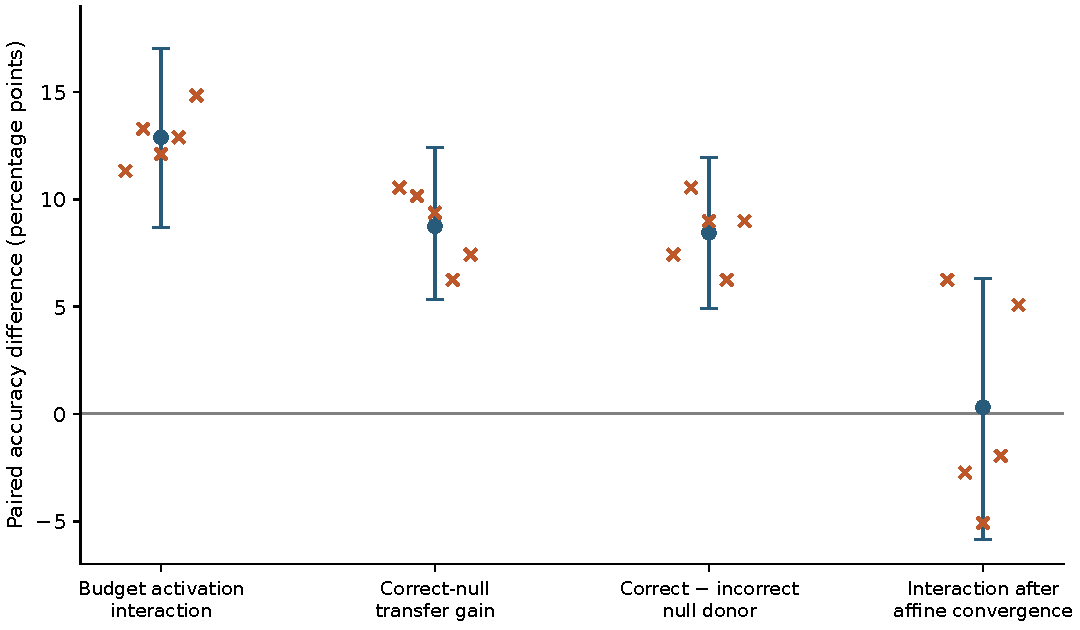
\includegraphics[width=.95\linewidth]{figures/final_contrasts.pdf}
\caption{All five source effects and descriptive crossed source/pair 95\% intervals for predeclared contrasts. Convergence narrows the original activation-by-correctness interaction.}\label{fig:contrasts}
\end{figure}

\subsection{Convergence and precision qualifications}
All twenty affine fits pass the registered convergence threshold. The largest independently recomputed training-objective gap bound is $3.87\times10^{-12}$.
The two initializations give identical compound classes; their largest first-state difference is $6.55\times10^{-5}$.
However, design condition numbers range from $8.65\times10^{7}$ to $1.29\times10^{8}$, and coefficient norms from $8.01\times10^{5}$ to $1.69\times10^{6}$.
Complete float32 replay of the affine, second-operator, and readout pipeline changes 12/1280 correct-pairing and 43/1280 incorrect-pairing collision predictions relative to float64.
Aggregate correct/incorrect accuracy is 19.92/8.36\% in float64 and 19.92/8.44\% in float32.
The aggregate correspondence benefit survives this precision check, while individual predictions are numerically sensitive.
LayerNorm's exact affine constraint makes finite-precision rank effects a remaining candidate explanation.
Convergence of the empirical objective does not guarantee numerically robust state identification or out-of-distribution stability.

\section{Supporting evidence and boundaries}
\subsection{Permutation correspondence and intermediate-state sufficiency}
The permutation task predicts the number of left-to-right maxima. Complement acts by $C(\pi)_j=n+1-\pi_j$ and inversion by $I(\pi)=\pi^{-1}$.
The main missing word is complement followed by inverse, with target readout at $I(C(\pi))$.
These experiments use a four-layer transformer and bidirectional involution supervision, rather than the matrix study's scalar encoder and forward-only operators.
Four correctness conditions and a matched 20-epoch no-geometry comparator are evaluated on the same collision test.
Six fitting repeats reuse three source initializations; they are not six independent source replications.

\begin{table}[ht]\centering
\begin{tabular}{lrr}\toprule
Geometric pairing & Collision accuracy(\%) & Pair double correctness(\%)\\\midrule
Both correct & 36.20 & 11.48\\
Complement correct only & 35.42 & 10.68\\
Inverse correct only & 30.92 & 5.68\\
Both matched incorrect & 29.87 & 4.30\\
No geometry, matched 20 epochs & 21.89 & 0.39\\\bottomrule
\end{tabular}
\caption{Same held-out 20-epoch permutation collision test. Geometric correctness changes only hidden pairing; all conditions retain correct output supervision.}\end{table}


Correct complement correspondence explains most of the factorial advantage; the extra inverse-correspondence increment is small and uncertain. The experiment does not support a required ordering of double-correct, either single-correct arm, and double-incorrect.
The 20-epoch fits continue 10-epoch optimizer states. The matched 20-epoch no-geometry comparator was added after observing the other 20-epoch outcomes, using the existing zero geometry weight without outcome-based tuning. This timing limits its confirmatory status.

The correct arm predicts the composition at 36.20\%, versus 93.35\% when the second operator receives the true intermediate. Repairing first-step readout-null error reaches 93.15\%, while repairing readout-row error reaches 59.09\%. These repairs require true intermediate states and are explanatory diagnostics. They are not deployable inference results. They motivated the final predicted-component transfers, which use no true intermediate.

\subsection{Initial affine cross-domain experiments}
Initial matrix and polynomial experiments use three ordinary sources, six adaptations per condition, and 900 fixed joint epochs in six conditions: the four correctness combinations, no geometry, and an output-space diagnostic.
All conditions keep correct native and generator-output supervision; output-space operators have fewer parameters and are not capacity-matched causal controls.
Matrix correct and incorrect composition scores are 9.44\% and 8.92\%, with a correct-minus-incorrect source-plus-whole-pair interval of $[-1.56,2.73]$ pp. True-intermediate composition reaches 99.22\%. Thus primitive answers and oracle composition can be reliable while a predicted intermediate is unusable.

For exact cubic polynomials over $\F_{13}$, translation $Tf(x)=f(x+1)$ and differentiation $Df=f'$ give visible answers $f(0),f(1),f'(0)$ and missing answer $f'(1)$. Here $DT=TD$; the task cannot establish order discrimination.
Correct and incorrect all-source accuracies are 8.27\% and 8.20\%.
Two of three sources miss the predefined 90\% translation threshold, so this failure cannot be cleanly attributed to composition alone.
The 128 pairs connect 39 derivative blocks into one component; they are not 128 independent block-level repetitions.
These studies provide boundaries, not a confirmed universal positive effect or a refutation of all irreversible relation learning.

\subsection{Why null information matters but null-only loss can fail}
A separate prospective intervention crosses full-space versus null-only loss with correct versus matched-incorrect targets, using three new source initializations in each domain.
The null-only objective is normalized in its own subspace and \emph{replaces} the full-space penalty.
It does not retain a full-space term and add null weighting.
The predeclared matrix interaction is $-1.30$ pp $[-5.08,2.60]$; the permutation interaction is $-5.57$ pp $[-10.31,-1.46]$.
This proposed loss replacement did not pass its confirmation.
Readout-null information can be important downstream while a null-only learning objective permits damaging row-space state error.

Finally, an earlier parameter-matched three-new-source matrix confirmation yielded a 14.71 pp $[9.51,20.05]$ interaction. Predicted-null transfers and affine convergence on those same sources were exploratory mechanisms, even when evaluated on fresh inputs. The five-new-source final study independently confirms the fixed hypotheses; these sources and outcomes are not pooled.

\section{Reviewer controls: state matching and interpretation}
These diagnostics were registered after the final confirmation, without changing any encoder, relation operator, or readout. We separately report previously inspected tests and a new set of 128 complete orbits (64 IID inputs and 32 collision pairs). The new orbits exclude training and validation of all five sources and every previously inspected test orbit. This is a small post-confirmation replication, not a new five-dataset study.

\paragraph{Predicted-state replication and distribution controls.}
On new collision pairs, the linear recipient reaches 10.00\%; correct predicted-null transfer reaches 15.31\%, versus 7.19\% for incorrect transfer. The difference is 8.125 points, with a descriptive crossed source/pair interval [1.25,15.625]; all five source differences are positive.
Validation-fitted mean/covariance transport of the incorrect donor reaches 7.50\%. This control addresses marginal null-coordinate distribution, not conditional state error, row/null dependence, or complete manifold membership.
Nearest-reference RMS distance is 0.565 for the correct hybrid, 0.616 for the incorrect hybrid, and 0.388 for true intermediate states. These distances concern natural training intermediates; they do not constitute a manifold-membership test. The distribution-shift explanation remains unresolved.

\paragraph{Error matching and its limitations.}
Within-input restriction to original correct/incorrect predictions whose null norms and errors both agree within 10\% retains only 3 source--sample observations; a 25\% restriction retains 18 of 320. The latter conditional difference is $-5.56$ points and is too sparse to support a stable mechanism conclusion. Conditioning on prediction error can remove a pathway through which correspondence acts; this is descriptive, not causal isolation.
An additional oracle diagnostic exactly matches each correct hybrid's null norm and error to the true intermediate, while preserving its row component. Reorienting a wrong donor yields 34.69\%, and randomized orientations yield 70.47\%. These controls use the true intermediate's direction. They are not learned predictions or evidence that wrong-pair training generalizes better. Their scope is narrower: equal scalar state error and norm do not imply equal downstream utility. Norm/error and marginal covariance controls are separate, rather than simultaneously matching all distributions.

\paragraph{Answers remain decodable from the null space.}
Independent ridge probes use support labels and known validation for regularization selection; they never update the composition pipeline. On true intermediate null coordinates, fresh-collision current-answer accuracy is 54.06\% (training-mode baseline 8.13\%) and future-answer accuracy is 52.81\%. Future labels are supplied only to these diagnostic probes. Thus the null component is invisible to one fixed linear readout, but is not independent of answer information.

\paragraph{Numerical audit.}
All five $13\times128$ readouts have numerical rank 13. SVD and pseudoinverse projectors agree; across every tested intervention and random draw, the maximum first-logit change is $4.11\times10^{-13}$. Norm/error matching discrepancies are below $1.14\times10^{-13}$. Independent reconstruction checks 499,530 sample/identity entries. These checks validate the defined interventions, not a natural relation-specific causal mechanism.

\begin{figure}[t]
\centering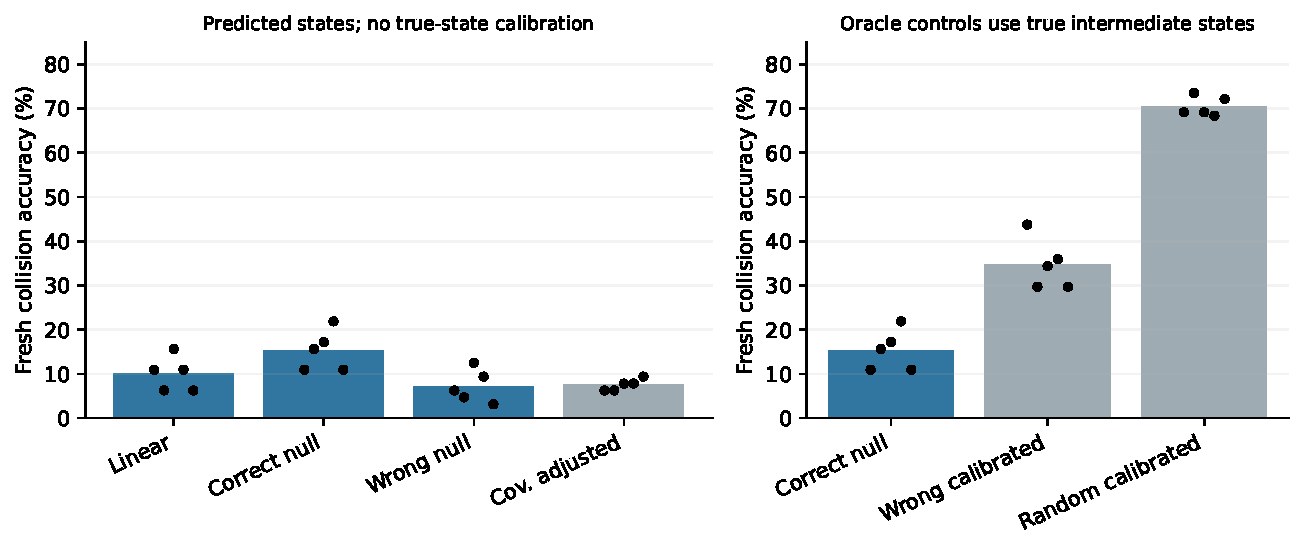
\includegraphics[width=\linewidth]{figures/reviewer_controls.pdf}
\caption{Frozen-model reviewer controls on new collision pairs. Dots show five source initializations, sharing test inputs. Right-hand calibrated controls use true intermediate states and are diagnostics only; they are not available predictors.}
\end{figure}

\section{Further reviewer revisions: scale and causal controls}
We retain the original correctness intervention, collision construction, complete-logit invariant swaps, and orbit exclusion. A post-confirmation census evaluates every unexposed orientation in each source's remaining 511--530 orbits, totaling 3,066--3,180 inputs per source. Independently paired collision inputs agree on all three visible gold answers and disagree on the compound answer. Each input is used once; complete orbits can recur across pairs. These are larger tests of old models, not new source/world replications.

\begin{table}[ht]\centering\small
\begin{tabular}{lrr}\toprule Condition & Accuracy (\%) & Both (\%)\\\midrule
nonlinear correct & 17.94 & 3.24 \\
nonlinear wrong & 7.46 & 0.48 \\
linear correct & 8.53 & 0.73 \\
linear wrong & 8.03 & 0.40 \\
affine correct ols initialization & 17.86 & 2.95 \\
affine wrong ols initialization & 7.44 & 0.53 \\
validation selected ridge correct & 11.19 & 1.19 \\
validation selected ridge wrong & 7.75 & 0.38 \\
\bottomrule\end{tabular}
\caption{Expanded gold-matched collision subset, averaged over the five old sources. Orbit dependencies remain.}
\end{table}

\paragraph{Equivalence remains secondary.}
On the complete orbit census the unregularized affine--GELU difference is 0.237pp; the descriptive 90\% source interval is $[-1.000,1.475]$pp. A posthoc paired TOST rejects non-equivalence for $\pm3$pp, whereas the original smaller test did not. This does not establish prospective equivalence on new data worlds. Normal-model planning with the old SD of 5.35pp requires 29 independent units for $\pm3$pp and 12 for $\pm5$pp at 80\% power if the true mean is zero; a 1pp true mean raises these to 46 and 14. The old variance is not a variance estimate for the new world. All equivalence analyses are secondary to the functionality question.

\paragraph{Ridge sensitivity weakens a broad optimization conclusion.}
We penalize standardized affine input coefficients, leaving the intercept unpenalized, and fit the same teacher-KD plus normalized-state objective with this added term. The ridge path is fixed before new predictions and selected only on known validation states/logits. Functional accuracy falls as small directions are suppressed; validation-selected fits perform poorly. Thus recovery by the unregularized solution is not robustly demonstrated under ordinary validation-selected regularization. This changes the empirical objective and cannot invalidate the original unregularized optimum certificate. The source of useful small directions remains unresolved.

\paragraph{Natural-state interchange is informative but not an ideal control.}
Balanced donor permutations preserve gold first answers and marginal donor frequency. With a distinct second answer, the natural donor is followed in 56.89\% of cases. With the same second answer, only 82.13\% remain correct and 18.25\% change predictions. All tested first-step logits remain invariant. The substantial same-answer disturbance fails the proposed near-invariant control, and natural components do not guarantee natural hybrids. The evidence supports downstream answer-information transport under the specified intervention, rather than natural mathematics-specific causal encoding. Geiger et al.'s interchange framework motivates the stronger prospective control \cite{geiger2021causal}.

\paragraph{A new-world confirmation is kept separate.}
The following section reports the completed frozen $\F_{17}$ experiment. Those independent dataset/source units are distinguished from the posthoc old-world census above. The interface-only parameter-count amendment was made before first-operator fitting or new composite evaluation, with both protocol versions retained. Failed performance and interchange gates are reported rather than used to replace units.

\begin{figure}[ht]\centering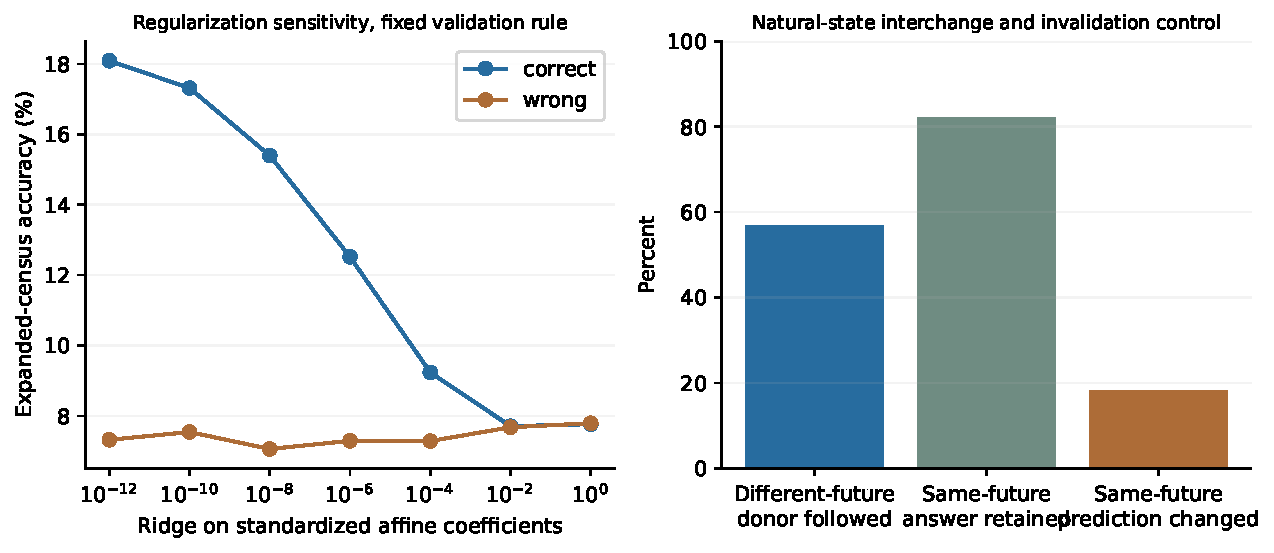
\includegraphics[width=\linewidth]{figures/reviewer_revision.pdf}
\caption{Complete-census regularization sensitivity and natural-state interchange. The same-answer disturbance prevents an unqualified causal-mechanism claim.}
\end{figure}

\section{Prospective confirmation in a new field and larger model}\label{sec:fresh}
The frozen new-world protocol was completed without inspecting any compound score during fitting. Seventeen independently sampled corpora, supports, validation sets, test sets and source initializations in $\F_{17}$ replace the shared old-world data. Each test contains 2,000 collision pairs and 512 IID inputs. The hidden width is 512 instead of 128. The joint encoder/generator preparation minibatch index stream retains the shared legacy scheduling code; data, model initialization and first/second-operator fitting streams vary. Randomly sampled units can overlap across units, but no weights are reused. This is one new algebraic system with independent random datasets, rather than 17 distinct systems.

\paragraph{Fixed design and two primary tests.}
Correct versus answer-matched incorrect first-step correspondence is crossed with the same parameter-matched Identity/GELU predictor. Correct output distillation, inputs, steps and encoder are identical within a unit. All 68 first predictors and 51 second-step noise candidates were fit before the test was opened. Second-step noise is chosen only by known single-step validation and is shared across the first-predictor arms. No compound label or compound target state enters training. The two predeclared source-level contrasts use paired two-sided $t$ tests with Holm correction; reported 95\% intervals are marginal rather than simultaneous.

GELU correct minus incorrect compound accuracy is 5.157 pp, with interval [1.924,8.391] pp and Holm $p=0.00381$. Natural null versus row interchange donor-target accuracy is 49.322 pp, with interval [43.527,55.117] pp and Holm $p=9.3\times10^{-12}$. Row interchange is a localization diagnostic that can change first logits; null interchange preserves them. All 17 units are retained.

\begin{table}[ht]\centering\small
\begin{tabular}{lrrrr}\toprule First predictor & Compound (\%) & Both (\%) & First (\%) & State MSE\\\midrule
linear correct & 6.75 & 0.34 & 99.96 & 0.1431 \\
linear wrong & 6.11 & 0.24 & 99.96 & 0.1968 \\
nonlinear correct & 11.52 & 1.52 & 99.95 & 0.0699 \\
nonlinear wrong & 6.36 & 0.27 & 99.96 & 0.2087 \\
\bottomrule\end{tabular}
\caption{Mean collision performance with the validation-selected second operator in the new field. Datasets and initializations both vary across the 17 statistical units.}
\end{table}

\paragraph{Error decomposition and the performance gate.}
The selected second operator reaches 99.73\% on true intermediate states, versus 11.52\% with correctly paired GELU predictions. The mean fraction of the oracle--incorrect gap closed is 5.53\%. This contrasts first-state error with downstream failure and does not treat first-answer accuracy as state sufficiency. The original second operator, all IID results and all individual units are also archived. The preregistered 40\% performance gate is not passed. No further candidate was selected by compound results.

\paragraph{Natural-state interchange and its invalidation control.}
Donors have the same first gold answer, lie in a different orbit and are used once per arm. Distinct-future null donors are followed in 52.02\%, compared with 2.70\% for distinct-future row donors. Same-future null donors retain the donor answer in 71.93\%, but change 28.10\% of predictions; the preregistered 5\% change gate is not passed. The maximum first-logit change for null interchange is $1.98\times10^{-13}$. Even natural components can yield off-manifold hybrids. These findings concern downstream answer-information transport, not identification of natural mathematics-specific relation coding.

\paragraph{Scope and equivalence.}
The larger model, increased input coverage, new field and noisy second-step fitting change together. This confirmation cannot isolate a width effect. It also does not fit the converged affine baseline in the new world; any finite-budget activation contrast is not a convergence or equivalence result. The old affine--GELU TOST analyses remain secondary and posthoc, with the primary wording ``additional advantage was not confirmed'' limited to the old unregularized diagnostic. Independent replay reconstructs 2,161,059 label, split, prediction and invariant entries; it validates the registered computation without strengthening its causal scope.

\begin{figure}[ht]\centering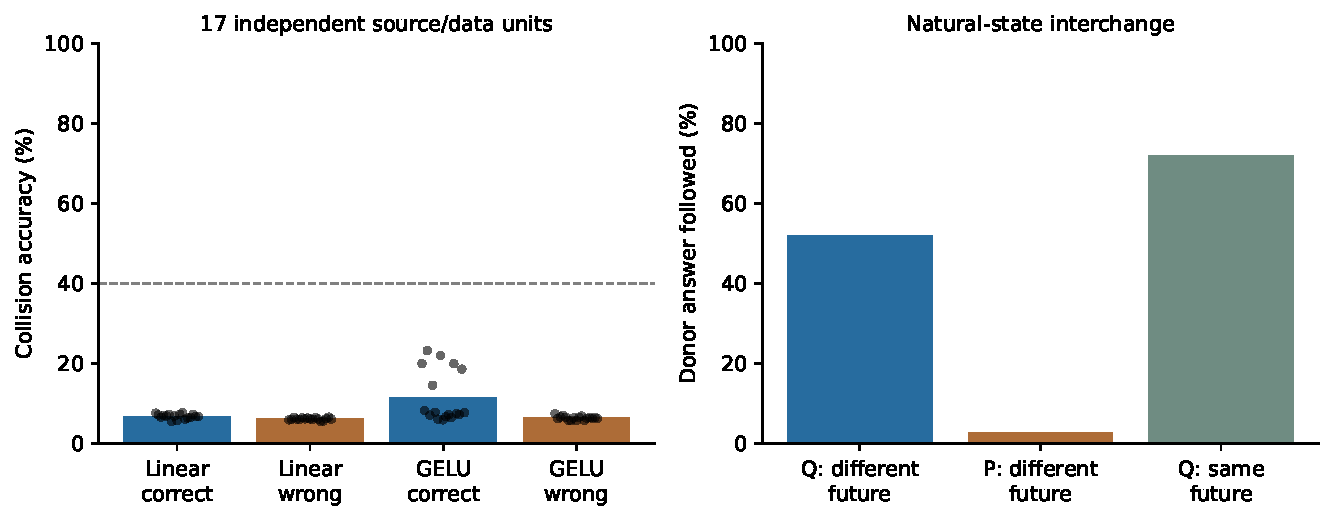
\includegraphics[width=\linewidth]{figures/reviewer_fresh.pdf}
\caption{Frozen new-field confirmation. Points are independent source/data units; the dashed line is the predeclared 40\% accuracy gate. Natural-state swaps address downstream information transport.}
\end{figure}

\section{Discussion and limitations}
The prospective new-field comparison measures a 5.157pp correctness benefit for GELU compound prediction, with marginal 95\% interval $[1.924,8.391]$ and Holm $p=0.00381$. Independent datasets and initializations replace the shared-data limitation of the earlier five-source comparison. The evidence remains conditional on correctly prepared encoders and this supplied correspondence intervention.

\paragraph{What the interventions identify.}
The readout-null projector concerns one fixed linear readout. It neither removes nonlinear answer information nor ensures independence from current or future answers; diagnostic probes recover both. Predicted-null transfer establishes a functional effect of the defined hybrid. Natural-state interchange supplies a more direct counterfactual information-transport check, but natural components can still produce off-manifold mixtures. In the new test same-future swaps change 28.10\% of predictions, and the fixed 5\% stability gate fails. This gate must accompany any donor-following result. The row-swap comparison is a localization diagnostic, not an intervention preserving all first-step logits. We do not identify the transferred content uniquely as mathematical relation information.

Correct versus incorrect hidden targets preserve gold answer triples and use the same soft output targets. They still change target-state consistency with those soft targets and the natural hidden-state distribution. Marginal covariance transport and sparse scalar-error matching do not eliminate conditional state-distribution explanations. Oracle error-calibrated random donors use true intermediate states and cannot be interpreted as available learned predictors.

\paragraph{Performance and generalization.}
New-field correct GELU accuracy is 11.52\%, compared with 99.73\% for true intermediates; the 40\% performance gate fails. High first-step accuracy does not guarantee a state that the second operator can use. Every registered unit and every failed gate is retained. Noise-candidate selection uses single-step validation only, and the original second operator is reported alongside the selected one. These changes were fixed before composite scores, not selected to repair an observed compound result.

The 17 source/data units come from independent random partitions of one new finite-field system; they are not 17 distinct algebraic systems. Cross-unit data overlap is permitted. Ordinary source training, initializations and predictor fitting have varying random streams; the joint-preparation batch-index stream retains a shared legacy schedule. The primary statistical unit is the dataset/source pair, with Holm adjustment for two predeclared tests. Old-world bootstrap and TOST analyses remain descriptive or secondary. Confidence intervals in the new report are marginal, not simultaneous. Width, coverage, field and second-step robustness change together; none is isolated as the sole cause of a performance change.

\paragraph{Optimization and numerical limits.}
Adequate unregularized affine fitting largely recovers the old-world nonlinear functional advantage; an additional advantage was not confirmed there. A zero-crossing interval is not an equivalence test. Expanded old-world TOST analyses are explicitly secondary and posthoc, and no converged affine fitting was performed in the new field. Validation-selected ridge fits lose much of the old affine benefit, preventing a broad claim that optimization explains away nonlinear advantages. Ridge changes the objective, so this loss does not invalidate the original unregularized optimum diagnostic.

Direct affine fitting changes parameterization, precision and budget. Ill-conditioned designs, large coefficients and tiny directions associated with LayerNorm's exact affine constraint leave numerical robustness unresolved. Empirical convergence does not bound held-out state error. No precise allocation of the effects to optimization, conditioning and expressivity is supported. The irreversible polynomial setting has primitive-generalization failures; different domain architectures and supervision directions prevent a universal algebra-based explanation.

\section{Conclusion}
Correct supplied state correspondence and compositional state sufficiency are separate from first-step answer accuracy. The fixed new-world study tests correspondence functionality and natural-state information transport with independent datasets, larger tests and two corrected primary comparisons. Earlier predicted-null and affine diagnostics reveal functional pathways while the ridge and same-answer controls restrict mechanistic claims. The paper reports the benefits, failed gates and numerical boundaries of these interventions; it does not equate detectable geometry with spontaneous or universal algebraic reasoning.

\bibliographystyle{plain}
\bibliography{references_revised}
\clearpage
\appendix
\section{Protocol details and evidence provenance}
The main text follows the argument rather than the chronological order of exploratory runs.
Immutable protocol, fit, test-opening, prediction, and delivery records retain that chronology.
Table~\ref{tab:studies} distinguishes the roles of the major studies.
The final five-source test was not used for hyperparameter or checkpoint selection. Its ending rule closed experiments after the predefined source, optimization, and precision checks, regardless of the result.

\begin{table}[ht]\centering\small
\begin{tabular}{p{.23\linewidth}p{.24\linewidth}p{.42\linewidth}}
\toprule Study & Sources / budget & Evidential role\\\midrule
Permutation factorial & 3 sources, 6 fits per arm; 20 epochs & Correspondence-sensitive composition; true-state localization is diagnostic.\\
Initial matrix/polynomial & 3 sources, 6 fits per arm; 900 joint epochs & Cross-domain boundaries; polynomial primitive failures retained.\\
Null-only replacement & 3 new sources per domain; 20 permutation or 900 matrix epochs & Prospective test of the specified replacement objective.\\
Activation confirmation & 3 new matrix sources; 2,000 updates & Parameter-matched confirmation with $10^{-4}$ decay.\\
Reused-source mechanisms & Same preceding 3 sources & Exploratory predicted-null and optimization diagnostics; not new-source replication.\\
Final confirmation & 5 new matrix sources; 20 budget fits, 20 affine solves & Fixed hypotheses independently checked; zero decay for the shared loss.\\
\bottomrule
\end{tabular}
\caption{Evidence roles and differences that prevent indiscriminate pooling.}\label{tab:studies}
\end{table}

\subsection{Data, initialization, and training}
The final seeds and partitions are stored in \texttt{configs/final\_mechanism\_confirmation.json}.
Source training has 512 anchors; known validation has 128 and pilot validation 64. Each first-operator support has 1,024 answer-stratified eligible anchors.
Numeric coordinates are centered at 6 and scaled by $2\pi/13$. The scalar encoder is Linear(4,128), GELU, Linear(128,128), and LayerNorm.
Ordinary training uses 500 epochs, batch size 128 and learning rate 0.003. Correct source preparation uses 900 joint epochs, batch size 64, encoder learning rate 0.0008 and operator learning rate 0.002.
The original readout is preserved during relation preparation. Native CE, native KD and generator-output KD have coefficient one; geometry has coefficient 0.25.
The final first-operator stage is separately specified in Section~3 and freezes these prepared models.

\subsection{State-error and null-transfer algebra}
The reported final first-state NMSE is
$\|\hat H_A-H_A\|_F^2/(Nds^2)$ with the training variance $s^2$ fixed across the four arms.
Initial cross-domain displacement NMSE uses actual displacement energy and is not numerically comparable to this variance normalization.
CKA is computed as an auxiliary centered-Gram similarity and is not an accuracy surrogate.

Let $P$ be the orthogonal projector onto the row span of $W$ and $Q=I-P$.
Then $QW^\top=0$ and the predicted hybrid
$\hat h_{L\leftarrow G}=\hat h_L+(\hat h_G-\hat h_L)Q$
satisfies $z(\hat h_{L\leftarrow G})=z(\hat h_L)$.
For an affine second operator $R_B(h)=hM_B+b_B$, the final logit difference is
$(\hat h_G-\hat h_L)QM_BW^\top$, which need not vanish.
Thus invisibility to the first readout is consistent with downstream usefulness.
This algebra alone does not imply that the transferred state is correct; the held-out intervention measures that.

For first-step error $e=\hat h_A-h_A$, the composition error decomposes as
$eM_B+[R_B(h_A)-h_{AB}]$.
Its squared norm includes a cross term. Propagated row/null energies and oracle repairs must not be interpreted as additive causal percentages.

\subsection{Same-family convex optimization}\label{app:convergence}
A width-256 Identity residual can express any affine residual on dimension 128; adding the frozen affine skip retains the unrestricted affine family.
With the augmented training design $X=[H_0,\mathbf{1}]$, retain all singular directions above the registered $10^{-12}$ relative threshold.
All final designs retain 129 directions.
Use $F=\sqrt{N}U$, so $F^\top F/N=I$, and express predictions as $FC$.
The readout-null coefficients minimizing Equation~\ref{eq:loss} are their least-squares solution because KD is invariant to those coefficients.
Readout-row coefficients are fitted using float64 L-BFGS (history 100, maximum 2,000 iterations, gradient tolerance $10^{-9}$, change tolerance $10^{-14}$, strong-Wolfe search).
OLS and budget-linear row initializations are both fixed beforehand.

The quadratic term has Hessian $2\lambda I/(ds^2)$ in whitened coefficient coordinates and KD is convex in logits.
Writing $\mu=2\lambda/(ds^2)$, strong convexity gives
\[
 L(C)-L(C^\star)\leq\frac{\|\nabla L(C)\|_F^2}{2\mu}.
\]
The implementation independently recomputes the full analytic gradient, including null coordinates, and evaluates this bound in float64.
These are numerically computed empirical-objective diagnostics, not interval-arithmetic proofs.
The registered acceptable bound is $10^{-8}$.
No ridge, changed teacher targets, altered loss weights, or compound outcomes enter the solve.

\subsection{Collision ceilings and information controls}
On a pair with the same visible gold-answer triple and different compound labels, a deterministic predictor using only that triple must give the same answer to both inputs. Its pairwise double-correct rate is zero and aggregate pair accuracy is at most 50\%.
These ceilings do not apply to full probability outputs, hidden states, or input features. Positive pairwise success alone therefore does not establish an output-independent mechanism. We do not claim to surpass the 50\% ceiling stably.

\subsection{Supporting-study selection and dependence}
The initial one-hot/numeric matrix encoder fit generator outputs but generalized poorly. The scalar encoder was selected using known-state validation, including a reserved confirmation set, before compound testing; the polynomial study reused that architecture.
This feasibility stage precedes the cross-domain protocol and is not itself a new confirmatory test.
The permutation 20-epoch continuation and later no-geometry comparator are explicitly dependent or posthoc, respectively.
Polynomial splitting audits the actual observed and evaluated paths. Full semigroup-closure separation is impossible because $D^4$ maps all cubics to zero.
Source-only polynomial intervals condition on the shared test set and cannot convert its connected collision graph into independent input replications.

\section{Reproducibility and literature audit}
The public repository contains the experiment implementations, fixed configurations, tests, readable results, original sealed delivery manifests, and this revised manuscript.
Downloadable archives preserve the main experiment inputs, predictions and checkpoints; archive inventories and checksums identify exactly what is included.
A portable verifier resolves recorded historical workspace paths and runs replay in a temporary copy, preserving the sealed artifacts.
The numerical results in the revised tables are generated from completed JSON records, without retraining or selecting new outcomes.
The prior 174-test run and independent final replay are distinct verification evidence; test counts do not constitute statistical replications.

The literature audit records twelve original studies with exact titles, venues, primary URLs, source locators, and claim-level relevance in \texttt{paper/literature\_review.csv}.
It is a targeted review of the closest mechanisms and controls, not an assertion that no other related study exists.
No new priority or first-discovery claim is inferred from the search.

\section{Source-level results and the complete contrast inventory}
\begin{table}[ht]\centering\small
\begin{tabular}{lrrrrrr}\toprule
Source seed & L correct & L wrong & G correct & G wrong & Affine correct & Correct-null swap\\\midrule
17291 & 8.20 & 8.59 & 19.92 & 8.98 & 15.23 & 18.75 \\
18401 & 8.20 & 8.98 & 21.09 & 8.59 & 24.61 & 18.36 \\
19507 & 7.42 & 9.38 & 17.58 & 7.42 & 22.27 & 16.80 \\
20611 & 8.20 & 9.38 & 18.75 & 7.03 & 20.70 & 14.45 \\
21713 & 10.16 & 10.94 & 24.22 & 10.16 & 16.80 & 17.58 \\
\bottomrule\end{tabular}
\caption{Collision AB accuracy (\%) for every final source. All ten affine cases also include the second fixed solver initialization in the archived results.}
\end{table}
\begin{table}[ht]\centering\small
\begin{tabular}{lrr}\toprule
Accuracy contrast & Mean (pp) & Descriptive 95\% interval\\\midrule
gelu\_relation\_advantage & +11.88 & [+8.05,+15.62] \\
linear\_relation\_advantage & -1.02 & [-3.75,+1.80] \\
same\_budget\_interaction & +12.89 & [+8.67,+17.03] \\
correct\_null\_swap\_gain & +8.75 & [+5.31,+12.42] \\
correct\_vs\_wrong\_null\_donor & +8.44 & [+4.92,+11.95] \\
wrong\_null\_swap\_gain & +0.31 & [-2.73,+3.44] \\
remove\_correct\_gelu\_null & +7.11 & [+3.75,+10.55] \\
converged\_linear\_relation\_advantage & +11.56 & [+6.56,+16.80] \\
remaining\_relation\_interaction & +0.31 & [-5.86,+6.33] \\
converged\_linear\_vs\_gelu & -0.39 & [-6.09,+5.08] \\
linear\_optimization\_gain & +11.48 & [+6.56,+16.56] \\
\bottomrule\end{tabular}
\caption{All recorded final accuracy contrasts, including secondary explanatory contrasts. These are not eleven independent confirmatory tests.}
\end{table}
\section{Initial cross-domain outcome tables}
The following tables preserve the initial joint affine outcomes. Their six adaptation repeats reuse three sources. They are separate from the five-source frozen-encoder confirmation.
\paragraph{Matrix.}
\begin{center}\begin{tabular}{lrr}\toprule Condition & Accuracy(\%) & Double correct(\%)\\\midrule
both correct & 9.44 & 0.52\\
a correct b wrong & 8.66 & 0.39\\
a wrong b correct & 7.94 & 0.26\\
both wrong & 8.92 & 0.39\\
no geometry & 7.55 & 0.26\\
output space & 7.23 & 0.26\\
\bottomrule\end{tabular}\end{center}
All 36 models have the same 900-epoch budget. Source-cluster uncertainty conditions on the shared test inputs. Output-space results are information diagnostics with fewer parameters.
Correct-vs-incorrect collision accuracy differs by 0.52 percentage points; supplementary source-plus-whole-pair resampling gives[-1.56,2.73] percentage points. Thus a stable additional functional benefit is not established. Single-step scores are high, and true-intermediate prediction reaches 99.22\%, whereas inferred composition reaches9.44\%.
\paragraph{Polynomial.}
\begin{center}\begin{tabular}{lrr}\toprule Condition & Accuracy(\%) & Double correct(\%)\\\midrule
both correct & 8.27 & 0.39\\
a correct b wrong & 8.20 & 0.52\\
a wrong b correct & 8.20 & 0.65\\
both wrong & 8.20 & 0.39\\
no geometry & 6.77 & 0.13\\
output space & 7.36 & 0.26\\
\bottomrule\end{tabular}\end{center}
All 36 models have the same 900-epoch budget. Source-cluster uncertainty conditions on the shared test inputs. Output-space results are information diagnostics with fewer parameters.
The all-source correct group reaches 8.27\% versus8.20\% for incorrect geometry. Translation generator scores are91.80\%,87.11\%,87.50\% across sources; only the first meets the previously fixed90\% threshold. Its composition accuracy is7.42\%. Thus neither stable relation-specific benefit nor robust irreversible composition is established. Differentiation at the true intermediate achieves99.87\% overall.
The 128 collision pairs connect39 derivative blocks into one connected component. They cannot be treated as128 independent block-level repetitions; source intervals condition on this fixed test set.

\end{document}
